\documentclass{assignment}

\usepackage{float}
\usepackage{tikz}
\usepackage{adjustbox}
\usepackage{titlesec}
\usepackage{soul}
\usepackage{csvsimple}

\usepackage{graphicx}
\usepackage{subcaption}

\usetikzlibrary{calc,patterns,angles,quotes}
\setlength{\parindent}{0pt}

\hypersetup{
pdftitle={ME663 - Computational Fluid Dynamics},
pdfsubject={Report for assignment 1},
pdfauthor={Tommaso Bocchietti}
}

\makeglossaries

\newacronym{cfd}{CFD}{Computational Fluid Dynamics}
\newacronym{uds}{UDS}{Upwind Differencing Scheme}
\newacronym{quick}{QUICK}{Quadratic Upstream Interpolation for Convective Kinematics}
\newacronym{scgs}{SCGS}{Symmetric Coupled Gauss-Seidel}
\newacronym{sim}{SIMPLE}{Semi-Implicit Method for Pressure Linked Equations}

\begin{document}
\graphicspath{{./img/}}


\title{ME663 - Computational Fluid Dynamics \\ Assignment 1}
\author{Tommaso Bocchietti}
\date{A.Y. 2023/24 - W24}

\maketitle

\begin{figure}[H]
    \centering
    
\includegraphics[width=.9\textwidth]{./pdf/UniversityOfWaterloo_logo_vert_pms}
    \label{fig:University_Of_Waterloo_logo}
\end{figure}

\clearpage
\tableofcontents
\listoffigures
\listoftables
\printglossary[type=\acronymtype]

\clearpage
\section{Requests}
\label{sec:requests}

A system of two aluminum bars of the same material is shown in the following figure.
The system is subjected to two external loads, $P_x$ and $P_y$, at joint B.
A and C are connected to pinned supports.

\begin{figure}[h]
    \centering
    \begin{tikzpicture}[scale=3]

        \coordinate (A) at (0,0.5);
        \coordinate (B) at (3,0.5);
        \coordinate (Bf) at (3.7,1);
        \coordinate (C) at (3,0);

        % Joint names
        \node at (A) [above, left] {A};
        \node at (B) [below, above] {B};
        \node at (C) [below, left] {C};

        % Initial position
        \draw (A) -- (B) node[midway, below] {$L_1$};
        \draw (C) -- (B) node[midway, left] {$L_2$};

        % Deformed position
        \draw[dashed] (A) -- (Bf)node[midway, above] {$l_1$};
        \draw[dashed] (C) -- (Bf)node[midway, right] {$l_2$};

        % Labels
        \pic [draw, ->, "$\alpha$", angle radius=2cm] {angle = B--A--Bf};
        \pic [draw, <-, "$\beta$", angle radius=0.7cm] {angle = Bf--C--B};

        % Support at the end of Beam 1
        \draw[fill] (0,0.5) circle (0.03);

        % Support at the end of Beam 2
        \draw[fill] (3,0) circle (0.03);

        % Arrows at coordinate Bf
        \draw[->] (Bf) -- ++(0.3, 0) node[right] {$\vec{P_x}$};
        \draw[->] (Bf) -- ++(0, 0.3) node[above] {$\vec{P_y}$};
        \draw[->] (B) -- (Bf) node[midway, above] {$\vec{u}$};
        % \draw[->, shorten >=150pt] (Bf) -- (A) node[above, above] {$\vec{F_1}$};
        % \draw[->, shorten >=50pt] (Bf) -- (C) node[above, right] {$\vec{F_2}$};

    \end{tikzpicture}
    \caption{Problem representation}
    \label{fig:problem_representation}
\end{figure}

The problem asks to:

\begin{itemize}
    \item Obtain the external loads $P_x$ and $P_y$ as a function of horizontal and vertical displacements at point B (namely $u$ and $v$).
    \item Determine the displacements in both $x$ and $y$ directions for $1000$ load increments of $+5\text{N}$ for both $P_x$ and $P_y$ (from zero).
    \item Find the displacement of point B after the final increment.
\end{itemize}

Write a \texttt{MATLAB} code with a convergence error of $10^-5$ to numerically solve the problem.
Use a combination of (a) Euler and N-R, and (b) Euler and modified N-R.
Also plot the resultant force versus the resultant displacement.

Use the Green strain measure:

\begin{equation}
    E_i = \frac{l_i^2 - L^2}{2L^2}
    \label{eq:green_strain_measure_formula}
\end{equation}

From now on, we will refer to the Green strain measure as $\epsilon_{1,2}$ to differentiate it from the Young's modulus $E_{1,2}$.

\begin{table}[H]
    \centering
    \begin{tabular}{|c|c|c|}
        \hline
        \textbf{Parameter} & \textbf{Value} & \textbf{Unit} \\ \hline
        $E_1 = E_2 = E$    & $70$           & $\text{GPa}$  \\ \hline
        $L_1$              & $3$            & $\text{m}$    \\ \hline
        $L_2$              & $0.5$          & $\text{m}$    \\ \hline
        $A_1 = A_2 = A$    & $0.0001$       & $\text{m}^2$  \\ \hline
    \end{tabular}
    \caption{Parameters of the system}
    \label{tab:parameters_of_the_system}
\end{table}

\section{Methods}
\label{sec:methods}

\paragraph{Research Methodology}
The research will be conducted through a literature review of scientific articles, conference papers and thesis if available.
The main sources of information will be the IEEE Xplore, ScienceDirect, and Google Scholar databases.
The search will be conducted using the following keywords: "Chip-Scale Atomic Clock", "Atomic Clock", "MEMS", "CSAC", "Vapor Cell", "Rubidium", "Cesium", "Microwave Cavity", "Laser Cooling", "Photon Detector", "Quartz Crystal Oscillator", "Electron Spin", "Electron Excitation", "Optical Lattice Clock", "Quantum Technologies".

During the research, we will try to annotate the most relevant papers and articles, that will be then used to write the final report.

\paragraph{Outline}
We leave here a general outline that will be used as a guide for the development of the project.

\begin{enumerate}
    \item Introduction: Discuss the need for precise timekeeping and the exigence of chip-scale atomic clocks.
    \item \textbf{Engineering of Chip-Scale Atomic Clocks}: Discuss the principles of operation. Note: It would be interesting to use simulation tools such as \texttt{COMSOL Multiphysics} to visualize the operating principles of these devices, but not knowing the software and its capabilities, I am not sure if it is applicable here.
          \begin{itemize}
              \item Vapour cell
              \item Magnetic selector (electron spin)
              \item Microwave cavity (electron excitation at hyperfine transition)
              \item Laser system (laser cooling and trapping of atoms)
              \item Photon detector
              \item Closed loop over quartz crystal oscillator
          \end{itemize}
          \begin{figure}[H]
              \centering
              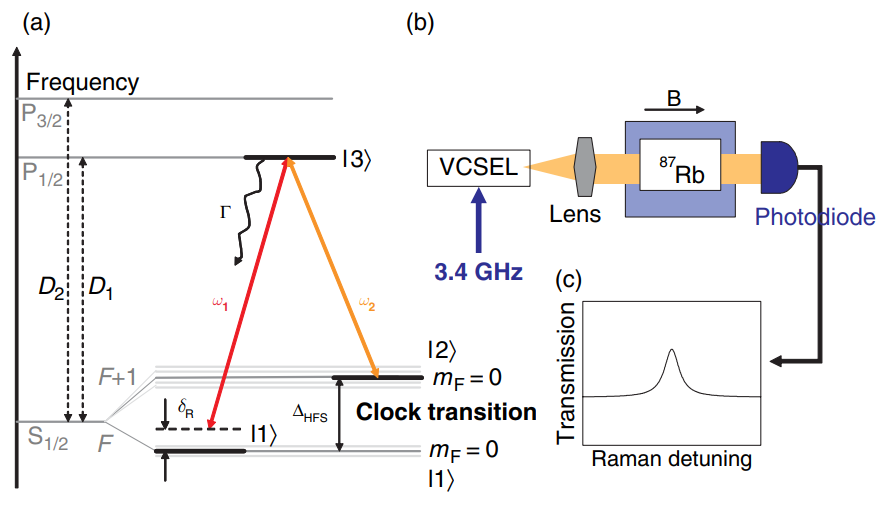
\includegraphics[width=.6\textwidth]{img/atomic_clock_logic}
              \caption{Schematic of the simplified atomic energy level configuration \cite{KNAPPE2008571}}
          \end{figure}

    \item \textbf{Technology Comparison}: Introduce the different types of chip-scale atomic clocks. Compare and contrast the different chip-scale atomic clock technologies in terms of size, power consumption, accuracy, and suitability for various applications.
          \begin{itemize}
              \item Cesium based
              \item Rubidium based
          \end{itemize}
          % \item Fabrication and Manufacturing: Explore the components of chip-scale atomic clocks such as atomic vapor cells, laser systems, and control electronics. Understand the microfabrication techniques used in their manufacturing.
    \item Applications: Consider the diverse applications of chip-scale atomic clocks (aerospace and defense to telecommunications and scientific research)
    \item Challenges and Future Directions: Identify current challenges such as size reduction and power efficiency, and consider future trends like adoption of optical lattice clocks and integration with quantum technologies.
    \item Conclusion: Summarize the key findings of the research and discuss the implications for future advancements and applications of chip-scale atomic clocks.
\end{enumerate}

% In case of time availability, we will also cover the Fabrication and Manufacturing of these devices, understanding the microfabrication techniques used in their manufacturing.

\paragraph{Time schedule}
In general, given a time constraint of 4/5 weeks, the project will be divided as follows (tentative)

\begin{itemize}
    \item Week 1: Introduction + Engineering of Chip-Scale Atomic Clocks
    \item Week 2: Engineering of Chip-Scale Atomic Clocks (possible simulation and results analysis)
    \item Week 3: Technology Comparison + Applications
    \item Week 4: Challenges and Future Directions + Conclusion
    \item Week 5: Final report writing
\end{itemize}

\section{Derivation of discretized governing equations}
\label{sec:derivation_of_discretized_governing_equations}

In this section, we will derive the discretized governing equations for the incompressible Navier-Stokes equations, which will be used to solve the problem at hand.

The set of incompressible Navier-Stokes equations is given by:

\begin{equation*}
    \nabla \cdot {\mathbf{u}} = 0
    \label{eq:incompressible_navier_stokes_continuity}
\end{equation*}

\begin{equation*}
    \rho \frac{\partial \mathbf{u}}{\partial t} + \rho \mathbf{u} \cdot \nabla \mathbf{u} = -\nabla p + \mu \nabla^2 \mathbf{u} + \mathbf{f}
    \label{eq:incompressible_navier_stokes_momentum}
\end{equation*}

In the rest of the document, the following hypotheses will be considered:

\begin{itemize}
    \item Steady-state problem: $\frac{\partial \mathbf{u}}{\partial t} = 0$
    \item Constant density: $\rho = \text{const}$
    \item Constant dynamic viscosity: $\mu = \text{const}$
    \item Zero body forces: $\mathbf{f} = 0$
\end{itemize}

Based on these hypotheses, the incompressible Navier-Stokes equations can be simplified and expanded as follows:

\begin{align}
    \frac{\partial u}{\partial x} + \frac{\partial v}{\partial y}     & = 0                                                                                                                         \\
    \frac{\partial u u}{\partial x} + \frac{\partial v u}{\partial y} & = -\frac{\partial p}{\partial x} + \nu \left( \frac{\partial^2 u}{\partial x^2} + \frac{\partial^2 u}{\partial y^2} \right) \\
    \frac{\partial u v}{\partial x} + \frac{\partial v v}{\partial y} & = -\frac{\partial p}{\partial y} + \nu \left( \frac{\partial^2 v}{\partial x^2} + \frac{\partial^2 v}{\partial y^2} \right)
    \label{eq:incompressible_navier_stokes_steady_2D}
\end{align}

Where $\nu = \frac{\mu}{\rho}$ is the kinematic viscosity and $p = \frac{p}{\rho}$ is the non-dimensional pressure.

Obviously, to solve the problem using a discrete calculator, the equations must be therefore discretized.

\subsection{Finite Volume Method}
\label{subsec:finite_volume_method}

The Finite Volume Method (FVM) is a numerical technique used to discretize partial differential equations, and is particularly well suited for the discretization of the Navier-Stokes equations.

The idea here is to divide the domain into a set of control volumes, and then integrate the governing equations over each control volume.
The resulting set of equations will be a set of algebraic equations, which can be solved using a discrete calculator.


\subsubsection{Control volumes}

Before proceeding with the discretization of the governing equations, we need to define what a control volume is and the notations used in the rest of the document.

In particular, we will assume from now on to have a Cartesian grid, with a uniform mesh spacing in both the $x$ and $y$ directions.

From the Figure \ref{fig:control_volume}, we can appreciate graphically how the domain is divided.

\begin{figure}[H]
    \centering
    \def\nCV{5}
    \def\dX{1.5cm}
    \def\dY{1.5cm}
    \def\labelsH{{"WW", "W", "P", "E", "EE"}}
    \def\labelsV{{"SS", "S", "P", "N", "NN"}}

    \begin{tikzpicture}

        \foreach \n in {0,1,...,\nCV}
            {
                \draw (0, \n*\dY) -- (\nCV*\dX, \n*\dY);
                \draw (\n*\dX, 0) -- (\n*\dX, \nCV*\dY);
            }

        % \foreach \n in {0,1,...,\the\numexpr\nCV-1\relax}
        %     {
        %         \draw[dashed] (-\dX/2, \n*\dY + \dY/2) -- (\nCV*\dX+\dX/2, \n*\dY + \dY/2);
        %         \draw[dashed] (\n*\dX + \dX/2, -\dY/2) -- (\n*\dX + \dX/2, \nCV*\dY+\dY/2);
        %     }

        \foreach \y in {0,1,...,\the\numexpr\nCV-1\relax}
            {
                \foreach \x in {0,1,...,\the\numexpr\nCV-1\relax}
                    {
                        \node[font=\small] at (\x*\dX+\dX/6, \y*\dY+\dY/10) {$_{\the\numexpr\x+1\relax,\the\numexpr\y+1\relax}$};
                    }
            }

        \foreach \n in {0,1,...,\the\numexpr\nCV-1\relax}
            {
                \node[font=\small] at (\n*\dX+\dX/2, \nCV/2*\dY) {\pgfmathparse{\labelsH[\n]}\pgfmathresult};
                \node[font=\small] at (\nCV/2*\dX, \n*\dY+\dY/2) {\pgfmathparse{\labelsV[\n]}\pgfmathresult};
            }

        \node[font=\small] at (\nCV/2*\dX, \nCV/2*\dY+\dY/2) {$s$};
        \node[font=\small] at (\nCV/2*\dX, \nCV/2*\dY-\dY/2) {$n$};
        \node[font=\small] at (\nCV/2*\dX-\dX/2, \nCV/2*\dY) {$w$};
        \node[font=\small] at (\nCV/2*\dX+\dX/2, \nCV/2*\dY) {$e$};

        \fill[yellow, opacity=0.3] (\nCV/2*\dX-\dX/2, \nCV/2*\dY-\dY/2) rectangle (\nCV/2*\dX+\dX/2, \nCV/2*\dY+\dY/2);

    \end{tikzpicture}
    \caption{Control volumes and control volume faces.}
    \label{fig:control_volume}
\end{figure}

In particular, Figure \ref{fig:control_volume} shows:

\begin{itemize}
    \item A grid of control volumes, with the subscript $(i,j)$ indicating the position of the control volume in the $x$ and $y$ directions, respectively. For example, the control volume in the center of the grid has indices $(i,j)=(3,3)$.
    \item The control volume centers with capital letters, $P, N, S, E, W, \ldots$.
    \item The control volume faces with lowercase letters, $n, s, e, w$.
\end{itemize}

Notice also that the capital letters always refers to a relative position with respect to the control volume in consideration.
For example, $P$ refers to the control volume in consideration, $N$ refers to the control volume to the north of $P$, and so on.
For this reason, in Figure \ref{fig:control_volume}, the control volume $P$ is highlighted in yellow so to indicate that is the control volume in consideration.


\subsubsection{Staggered grid and $L_{shape}$}

As we will see later during the formulation of the solving solution, for the purpose of this work, we will use a specific type of grid, called staggered grid.

We can also give a brief definition of the two types of grids available in the literature, which are:

\begin{itemize}
    \item \textbf{Collocated grid}: all the variables are located at the same point in the control volume (e.g. the center of the control volume).
    \item \textbf{Staggered grid}: the variables are located at different points in the control volume (e.g. the velocity components are located at the center of the faces of the control volume, and the pressure is located at the center of the control volume).
\end{itemize}

Given the formulation of the staggered grid, it's now useful to define the so called $L_{shape}$, which is a frame used to define in a compact and clear way the position of the variables in the control volume.

The $L_{shape}$ has been reported for control volume $P$ in Figure \ref{fig:L_shape}.

\begin{figure}[H]
    \centering
    \def\nCV{3}
    \def\dX{3cm}
    \def\dY{3cm}
    \def\labelsH{{"W", "P", "E"}}
    \def\labelsV{{"S", "P", "N"}}

    \begin{tikzpicture}

        \foreach \n in {0,1,...,\nCV}
            {
                \draw (0, \n*\dY) -- (\nCV*\dX, \n*\dY);
                \draw (\n*\dX, 0) -- (\n*\dX, \nCV*\dY);
            }

        \foreach \n in {0,1,...,\the\numexpr\nCV-1\relax}
            {
                \draw[dashed] (-\dX/2, \n*\dY + \dY/2) -- (\nCV*\dX+\dX/2, \n*\dY + \dY/2);
                \draw[dashed] (\n*\dX + \dX/2, -\dY/2) -- (\n*\dX + \dX/2, \nCV*\dY+\dY/2);
            }

        \foreach \y in {0,1,...,\the\numexpr\nCV-1\relax}
            {
                \foreach \x in {0,1,...,\the\numexpr\nCV-1\relax}
                    {
                        \node[font=\small] at (\x*\dX+\dX/10, \y*\dY+\dY/15) {$_{\the\numexpr\x-(\nCV-1)/2\relax,\the\numexpr\y-(\nCV-1)/2\relax}$};
                    }
            }

        \foreach \n in {0,1,...,\the\numexpr\nCV-1\relax}
            {
                \node[font=\small] at (\n*\dX+\dX/2, \nCV/2*\dY) {\pgfmathparse{\labelsH[\n]}\pgfmathresult};
                \node[font=\small] at (\nCV/2*\dX, \n*\dY+\dY/2) {\pgfmathparse{\labelsV[\n]}\pgfmathresult};
            }

        \draw[thick, blue, ->] (\nCV/2*\dX, \nCV/2*\dY)++(0,  \dY/4) -- ++(0, \dY/2) node[pos=1, right] {$u_s$};
        \draw[thick, blue, ->] (\nCV/2*\dX, \nCV/2*\dY)++(0, -\dY/2-\dY/4) -- ++(0, \dY/2) node[pos=1, right] {$u_s$};
        \draw[thick, red, ->] (\nCV/2*\dX, \nCV/2*\dY)++(\dX/4, 0) -- ++(\dX/2, 0) node[pos=1, above] {$u_e$};
        \draw[thick, red, ->] (\nCV/2*\dX, \nCV/2*\dY)++(-\dX/2-\dX/4, 0) -- ++(\dX/2, 0) node[pos=1, above] {$u_w$};

        \fill[yellow, opacity=0.3] (\nCV/2*\dX-\dX/2, \nCV/2*\dY-\dY/2) rectangle (\nCV/2*\dX+\dX/2, \nCV/2*\dY+\dY/2);

    \end{tikzpicture}
    \caption{$L_{shape}$ for control volume $P$.}
    \label{fig:L_shape}
\end{figure}

Basically, the $L_{shape}$ for control volume $P$ links the velocity components to the control volume $P$ itself, and it's used to define the indexes of the system.

In particular, the same Figure \ref{fig:L_shape} can be represented using the index notations, as shown in Figure \ref{fig:L_shape_index}.

\begin{figure}[H]
    \centering
    \def\nCV{1}
    \def\dX{5cm}
    \def\dY{5cm}

    \begin{tikzpicture}[every node/.style={font=\huge}]

        \draw (0, 0) -- (\dX, 0) -- (\dX, \dY) -- (0, \dY) -- cycle;

        \node at (\dX/7, \dY/10) {$i,j$};

        \node at (\dX/2, \dY/2) {$P_{i,j}$};

        \draw[thick, blue, ->] (\dX/2, \dY/2)++(0,  \dY/4) -- ++(0, \dY/2) node[pos=1, right] {$u_{i,j}$};
        \draw[thick, blue, ->] (\dX/2, \dY/2)++(0, -\dY/2-\dY/4) -- ++(0, \dY/2) node[pos=1, right] {$u_{i,j-1}$};
        \draw[thick, red, ->] (\dX/2, \dY/2)++(\dX/4, 0) -- ++(\dX/2, 0) node[pos=1, above] {$u_{i,j}$};
        \draw[thick, red, ->] (\dX/2, \dY/2)++(-\dX/2-\dX/4, 0) -- ++(\dX/2, 0) node[pos=1, above] {$u_{i-1,j}$};

        \draw[yellow,
            opacity=0.3,
            line cap=round,
            double=yellow,
            double distance=\dX/5,
        ] (\dX/2, \dY/2) -- ++(0, \dY/2+\dY/4);

        \draw[yellow,
            opacity=0.3,
            line cap=round,
            double=yellow,
            double distance=\dX/5,
        ] (\dX/2, \dY/2) -- ++(\dX/2+\dX/4, 0);

        \draw[dashed, |-|] (0, -\dY/6) -- (\dX, -\dY/6) node[pos=1, below, font=\Large] {$\Delta x$};
        \draw[dashed, |-|] (-\dX/6, 0) -- (-\dX/6, \dY) node[pos=1, left, font=\Large] {$\Delta y$};

    \end{tikzpicture}
    \caption{$L_{shape}$ for control volume $P$ using index notations.}
    \label{fig:L_shape_index}
\end{figure}

From Figure \ref{fig:L_shape_index}, we can appreciate how the $L_{shape}$ works well with index notations, and can be useful when working purely with indexes to refer to the variables.
\subsection{Application of the Finite Volume Method}
\label{subsec:application_of_the_finite_volume_method}

Having defined our working framework, we can now proceed to the application of the Finite Volume Method (FVM) to the incompressible Navier-Stokes equations \ref{eq:incompressible_navier_stokes_steady_2D}.

To do so, we start by giving the general integral form of the governing equations, and then proceed to the discretization of the convection, diffusion and source terms separately.

In particular, assuming from now on to have a Cartesian grid, with a uniform mesh spacing in both the $x$ and $y$ directions, the (FVM) reads as follows:




From now on, we will focus on the $x$ direction, given that the treatment for the $y$ direction is analogous.

The first step is to integrate the governing equations over each control volume.

Our discretized set of equations will be:

\begin{align}
    % TODO Check if the equation is correct
    \int_{V} u \frac{\partial u}{\partial x} dV + v \frac{\partial u}{\partial y} dV - \frac{1}{\rho} \frac{\partial p}{\partial x} dV - \nu \left( \frac{\partial^2 u}{\partial x^2} + \frac{\partial^2 u}{\partial y^2} \right) dV - f_x dV = 0 \\
    \int_{V} u \frac{\partial v}{\partial x} dV + v \frac{\partial v}{\partial y} dV - \frac{1}{\rho} \frac{\partial p}{\partial y} dV - \nu \left( \frac{\partial^2 v}{\partial x^2} + \frac{\partial^2 v}{\partial y^2} \right) dV - f_y dV = 0
\end{align}

We can now proceed to the discretization of the convection, diffusion and source terms separately.

The rest of the treatment will be done considering just the $x$ direction, given that the treatment for the $y$ direction is analogous.

Our starter equation is:

\begin{equation}
    \int_{V} \underbrace{u \frac{\partial u}{\partial x} + v \frac{\partial u}{\partial y}}_{\text{Convection term}} - \underbrace{\frac{1}{\rho} \frac{\partial p}{\partial x} dV}_{\text{Pressure term}} - \underbrace{\nu \left( \frac{\partial^2 u}{\partial x^2} + \frac{\partial^2 u}{\partial y^2} \right) dV}_{\text{Diffusion term}} - \underbrace{f_x dV}_{\text{Source term}} = 0
    \label{eq:inc_navier_stokes_steady_2D_discretized_x}
\end{equation}

Before proceeding, we need to define the control volume and the control volume faces geometrically.



% \subsection{Convection term}
\label{subsec:convection_term}
% \subsection{Diffusion term}
\label{subsec:diffusion_term}
% \subsection{Source term}
\label{subsec:source_term}
% \input{src/03.4 - discretized_governing_equations}


% \input{src/04 - derivation_of_discretized_boundary_condition_equations}

\clearpage
\bibliographystyle{plain}
\bibliography{ref}

% \clearpage
% \appendix
% \section{Mathematica code}
% \label{sec:appendix}

% Here follows the \texttt{Mathematica} notebook used for symbolic analysis of the equations.

% \lstinputlisting[
%     style=mathematica,
%     language=Mathematica,
%     caption=Mathematica notebook used for symbolic analysis of the equations.,
%     firstline=1,
%     lastline=56
% ]{files/notebook.txt}


\end{document}
